\documentclass[1p]{elsarticle_modified}
%\bibliographystyle{elsarticle-num}

%\usepackage[colorlinks]{hyperref}
%\usepackage{abbrmath_seonhwa} %\Abb, \Ascr, \Acal ,\Abf, \Afrak
\usepackage{amsfonts}
\usepackage{amssymb}
\usepackage{amsmath}
\usepackage{amsthm}
\usepackage{scalefnt}
\usepackage{amsbsy}
\usepackage{kotex}
\usepackage{caption}
\usepackage{subfig}
\usepackage{color}
\usepackage{graphicx}
\usepackage{xcolor} %% white, black, red, green, blue, cyan, magenta, yellow
\usepackage{float}
\usepackage{setspace}
\usepackage{hyperref}

\usepackage{tikz}
\usetikzlibrary{arrows}

\usepackage{multirow}
\usepackage{array} % fixed length table
\usepackage{hhline}

%%%%%%%%%%%%%%%%%%%%%
\makeatletter
\renewcommand*\env@matrix[1][\arraystretch]{%
	\edef\arraystretch{#1}%
	\hskip -\arraycolsep
	\let\@ifnextchar\new@ifnextchar
	\array{*\c@MaxMatrixCols c}}
\makeatother %https://tex.stackexchange.com/questions/14071/how-can-i-increase-the-line-spacing-in-a-matrix
%%%%%%%%%%%%%%%

\usepackage[normalem]{ulem}

\newcommand{\msout}[1]{\ifmmode\text{\sout{\ensuremath{#1}}}\else\sout{#1}\fi}
%SOURCE: \msout is \stkout macro in https://tex.stackexchange.com/questions/20609/strikeout-in-math-mode

\newcommand{\cancel}[1]{
	\ifmmode
	{\color{red}\msout{#1}}
	\else
	{\color{red}\sout{#1}}
	\fi
}

\newcommand{\add}[1]{
	{\color{blue}\uwave{#1}}
}

\newcommand{\replace}[2]{
	\ifmmode
	{\color{red}\msout{#1}}{\color{blue}\uwave{#2}}
	\else
	{\color{red}\sout{#1}}{\color{blue}\uwave{#2}}
	\fi
}

\newcommand{\Sol}{\mathcal{S}} %segment
\newcommand{\D}{D} %diagram
\newcommand{\A}{\mathcal{A}} %arc


%%%%%%%%%%%%%%%%%%%%%%%%%%%%%5 test

\def\sl{\operatorname{\textup{SL}}(2,\Cbb)}
\def\psl{\operatorname{\textup{PSL}}(2,\Cbb)}
\def\quan{\mkern 1mu \triangleright \mkern 1mu}

\theoremstyle{definition}
\newtheorem{thm}{Theorem}[section]
\newtheorem{prop}[thm]{Proposition}
\newtheorem{lem}[thm]{Lemma}
\newtheorem{ques}[thm]{Question}
\newtheorem{cor}[thm]{Corollary}
\newtheorem{defn}[thm]{Definition}
\newtheorem{exam}[thm]{Example}
\newtheorem{rmk}[thm]{Remark}
\newtheorem{alg}[thm]{Algorithm}

\newcommand{\I}{\sqrt{-1}}
\begin{document}

%\begin{frontmatter}
%
%\title{Boundary parabolic representations of knots up to 8 crossings}
%
%%% Group authors per affiliation:
%\author{Yunhi Cho} 
%\address{Department of Mathematics, University of Seoul, Seoul, Korea}
%\ead{yhcho@uos.ac.kr}
%
%
%\author{Seonhwa Kim} %\fnref{s_kim}}
%\address{Center for Geometry and Physics, Institute for Basic Science, Pohang, 37673, Korea}
%\ead{ryeona17@ibs.re.kr}
%
%\author{Hyuk Kim}
%\address{Department of Mathematical Sciences, Seoul National University, Seoul 08826, Korea}
%\ead{hyukkim@snu.ac.kr}
%
%\author{Seokbeom Yoon}
%\address{Department of Mathematical Sciences, Seoul National University, Seoul, 08826,  Korea}
%\ead{sbyoon15@snu.ac.kr}
%
%\begin{abstract}
%We find all boundary parabolic representation of knots up to 8 crossings.
%
%\end{abstract}
%\begin{keyword}
%    \MSC[2010] 57M25 
%\end{keyword}
%
%\end{frontmatter}

%\linenumbers
%\tableofcontents
%
\newcommand\colored[1]{\textcolor{white}{\rule[-0.35ex]{0.8em}{1.4ex}}\kern-0.8em\color{red} #1}%
%\newcommand\colored[1]{\textcolor{white}{ #1}\kern-2.17ex	\textcolor{white}{ #1}\kern-1.81ex	\textcolor{white}{ #1}\kern-2.15ex\color{red}#1	}

{\Large $\underline{12a_{1169}~(K12a_{1169})}$}

\setlength{\tabcolsep}{10pt}
\renewcommand{\arraystretch}{1.6}
\vspace{1cm}\begin{tabular}{m{100pt}>{\centering\arraybackslash}m{274pt}}
\multirow{5}{120pt}{
	\centering
	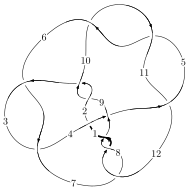
\includegraphics[width=112pt]{../../../GIT/diagram.site/Diagrams/png/1970_12a_1169.png}\\
\ \ \ A knot diagram\footnotemark}&
\allowdisplaybreaks
\textbf{Linearized knot diagam} \\
\cline{2-2}
 &
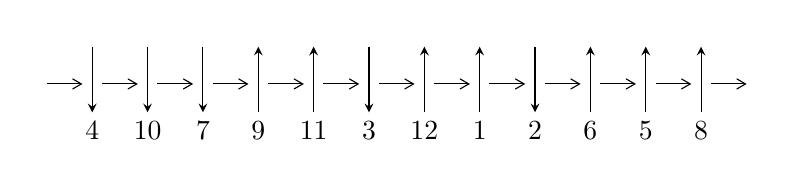
\begin{tikzpicture}[x=20pt, y=17pt]
	% nodes
	\node (C0) at (0, 0) {};
	\node (C1) at (1, 0) {};
	\node (C1U) at (1, +1) {};
	\node (C1D) at (1, -1) {4};

	\node (C2) at (2, 0) {};
	\node (C2U) at (2, +1) {};
	\node (C2D) at (2, -1) {10};

	\node (C3) at (3, 0) {};
	\node (C3U) at (3, +1) {};
	\node (C3D) at (3, -1) {7};

	\node (C4) at (4, 0) {};
	\node (C4U) at (4, +1) {};
	\node (C4D) at (4, -1) {9};

	\node (C5) at (5, 0) {};
	\node (C5U) at (5, +1) {};
	\node (C5D) at (5, -1) {11};

	\node (C6) at (6, 0) {};
	\node (C6U) at (6, +1) {};
	\node (C6D) at (6, -1) {3};

	\node (C7) at (7, 0) {};
	\node (C7U) at (7, +1) {};
	\node (C7D) at (7, -1) {12};

	\node (C8) at (8, 0) {};
	\node (C8U) at (8, +1) {};
	\node (C8D) at (8, -1) {1};

	\node (C9) at (9, 0) {};
	\node (C9U) at (9, +1) {};
	\node (C9D) at (9, -1) {2};

	\node (C10) at (10, 0) {};
	\node (C10U) at (10, +1) {};
	\node (C10D) at (10, -1) {6};

	\node (C11) at (11, 0) {};
	\node (C11U) at (11, +1) {};
	\node (C11D) at (11, -1) {5};

	\node (C12) at (12, 0) {};
	\node (C12U) at (12, +1) {};
	\node (C12D) at (12, -1) {8};
	\node (C13) at (13, 0) {};

	% arrows
	\draw[->,>={angle 60}]
	(C0) edge (C1) (C1) edge (C2) (C2) edge (C3) (C3) edge (C4) (C4) edge (C5) (C5) edge (C6) (C6) edge (C7) (C7) edge (C8) (C8) edge (C9) (C9) edge (C10) (C10) edge (C11) (C11) edge (C12) (C12) edge (C13) ;	\draw[->,>=stealth]
	(C1U) edge (C1D) (C2U) edge (C2D) (C3U) edge (C3D) (C4D) edge (C4U) (C5D) edge (C5U) (C6U) edge (C6D) (C7D) edge (C7U) (C8D) edge (C8U) (C9U) edge (C9D) (C10D) edge (C10U) (C11D) edge (C11U) (C12D) edge (C12U) ;
	\end{tikzpicture} \\
\hhline{~~} \\& 
\textbf{Solving Sequence} \\ \cline{2-2} 
 &
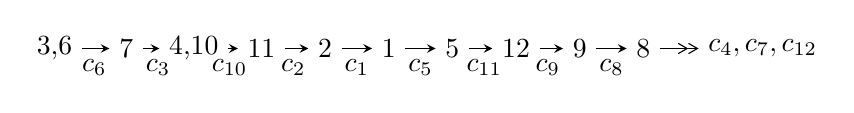
\begin{tikzpicture}[x=23pt, y=7pt]
	% node
	\node (A0) at (-1/8, 0) {3,6};
	\node (A1) at (1, 0) {7};
	\node (A2) at (33/16, 0) {4,10};
	\node (A3) at (25/8, 0) {11};
	\node (A4) at (33/8, 0) {2};
	\node (A5) at (41/8, 0) {1};
	\node (A6) at (49/8, 0) {5};
	\node (A7) at (57/8, 0) {12};
	\node (A8) at (65/8, 0) {9};
	\node (A9) at (73/8, 0) {8};
	\node (C1) at (1/2, -1) {$c_{6}$};
	\node (C2) at (3/2, -1) {$c_{3}$};
	\node (C3) at (21/8, -1) {$c_{10}$};
	\node (C4) at (29/8, -1) {$c_{2}$};
	\node (C5) at (37/8, -1) {$c_{1}$};
	\node (C6) at (45/8, -1) {$c_{5}$};
	\node (C7) at (53/8, -1) {$c_{11}$};
	\node (C8) at (61/8, -1) {$c_{9}$};
	\node (C9) at (69/8, -1) {$c_{8}$};
	\node (A10) at (11, 0) {$c_{4},c_{7},c_{12}$};

	% edge
	\draw[->,>=stealth]	
	(A0) edge (A1) (A1) edge (A2) (A2) edge (A3) (A3) edge (A4) (A4) edge (A5) (A5) edge (A6) (A6) edge (A7) (A7) edge (A8) (A8) edge (A9) ;
	\draw[->>,>={angle 60}]	
	(A9) edge (A10);
\end{tikzpicture} \\ 

\end{tabular} \\

\footnotetext{
The image of knot diagram is generated by the software ``\textbf{Draw programme}" developed by Andrew Bartholomew(\url{http://www.layer8.co.uk/maths/draw/index.htm\#Running-draw}), where we modified some parts for our purpose(\url{https://github.com/CATsTAILs/LinksPainter}).
}\phantom \\ \newline 
\centering \textbf{Ideals for irreducible components\footnotemark of $X_{\text{par}}$} 
 
\begin{align*}
I^u_{1}&=\langle 
3.52939\times10^{358} u^{88}-1.05772\times10^{359} u^{87}+\cdots+6.97081\times10^{361} b+7.41553\times10^{361},\\
\phantom{I^u_{1}}&\phantom{= \langle  }2.16674\times10^{361} u^{88}-7.26375\times10^{361} u^{87}+\cdots+7.24268\times10^{364} a-1.16875\times10^{366},\\
\phantom{I^u_{1}}&\phantom{= \langle  }u^{89}-2 u^{88}+\cdots+21705 u+1039\rangle \\
I^u_{2}&=\langle 
-14550 u^{20}+40621 u^{19}+\cdots+10007 b+23861,\\
\phantom{I^u_{2}}&\phantom{= \langle  }43297 u^{20}+522281 u^{19}+\cdots+590413 a+482394,\;u^{21}-3 u^{20}+\cdots-3 u+1\rangle \\
\\
\end{align*}
\raggedright * 2 irreducible components of $\dim_{\mathbb{C}}=0$, with total 110 representations.\\
\footnotetext{All coefficients of polynomials are rational numbers. But the coefficients are sometimes approximated in decimal forms when there is not enough margin.}
\newpage
\renewcommand{\arraystretch}{1}
\centering \section*{I. $I^u_{1}= \langle 3.53\times10^{358} u^{88}-1.06\times10^{359} u^{87}+\cdots+6.97\times10^{361} b+7.42\times10^{361},\;2.17\times10^{361} u^{88}-7.26\times10^{361} u^{87}+\cdots+7.24\times10^{364} a-1.17\times10^{366},\;u^{89}-2 u^{88}+\cdots+21705 u+1039 \rangle$}
\flushleft \textbf{(i) Arc colorings}\\
\begin{tabular}{m{7pt} m{180pt} m{7pt} m{180pt} }
\flushright $a_{3}=$&$\begin{pmatrix}0\\u\end{pmatrix}$ \\
\flushright $a_{6}=$&$\begin{pmatrix}1\\0\end{pmatrix}$ \\
\flushright $a_{7}=$&$\begin{pmatrix}1\\u^2\end{pmatrix}$ \\
\flushright $a_{4}=$&$\begin{pmatrix}- u\\- u^3+u\end{pmatrix}$ \\
\flushright $a_{10}=$&$\begin{pmatrix}-0.000299164 u^{88}+0.00100291 u^{87}+\cdots+83.3155 u+16.1369\\-0.000506310 u^{88}+0.00151735 u^{87}+\cdots-23.7024 u-1.06380\end{pmatrix}$ \\
\flushright $a_{11}=$&$\begin{pmatrix}-0.000805473 u^{88}+0.00252026 u^{87}+\cdots+59.6131 u+15.0731\\-0.000506310 u^{88}+0.00151735 u^{87}+\cdots-23.7024 u-1.06380\end{pmatrix}$ \\
\flushright $a_{2}=$&$\begin{pmatrix}-0.0000914777 u^{88}+0.000720740 u^{87}+\cdots+16.4384 u-11.3057\\-0.000933091 u^{88}+0.00300921 u^{87}+\cdots-3.26069 u-0.118984\end{pmatrix}$ \\
\flushright $a_{1}=$&$\begin{pmatrix}-0.00106155 u^{88}+0.00389260 u^{87}+\cdots+1.33023 u-12.0413\\-0.00154278 u^{88}+0.00499981 u^{87}+\cdots-13.8793 u-0.663133\end{pmatrix}$ \\
\flushright $a_{5}=$&$\begin{pmatrix}0.00102463 u^{88}-0.00409500 u^{87}+\cdots-107.112 u-0.571082\\0.000910114 u^{88}-0.00293287 u^{87}+\cdots+9.31770 u+0.203991\end{pmatrix}$ \\
\flushright $a_{12}=$&$\begin{pmatrix}-0.00290304 u^{88}+0.00870923 u^{87}+\cdots-80.1138 u+6.30898\\-0.00294118 u^{88}+0.00959789 u^{87}+\cdots-60.4307 u-3.05496\end{pmatrix}$ \\
\flushright $a_{9}=$&$\begin{pmatrix}-0.0000311348 u^{88}+0.00200854 u^{87}+\cdots+241.819 u+13.6918\\-0.000739385 u^{88}+0.00225940 u^{87}+\cdots-11.2394 u-0.123333\end{pmatrix}$ \\
\flushright $a_{8}=$&$\begin{pmatrix}0.00306576 u^{88}-0.00889713 u^{87}+\cdots+170.165 u+9.84182\\0.00288924 u^{88}-0.00941813 u^{87}+\cdots+49.9644 u+2.69032\end{pmatrix}$\\&\end{tabular}
\flushleft \textbf{(ii) Obstruction class $= -1$}\\~\\
\flushleft \textbf{(iii) Cusp Shapes $= 0.00522368 u^{88}-0.0168283 u^{87}+\cdots+167.584 u+9.76277$}\\~\\
\newpage\renewcommand{\arraystretch}{1}
\flushleft \textbf{(iv) u-Polynomials at the component}\newline \\
\begin{tabular}{m{50pt}|m{274pt}}
Crossings & \hspace{64pt}u-Polynomials at each crossing \\
\hline $$\begin{aligned}c_{1}\end{aligned}$$&$\begin{aligned}
&u^{89}-10 u^{88}+\cdots-12 u+1
\end{aligned}$\\
\hline $$\begin{aligned}c_{2},c_{9}\end{aligned}$$&$\begin{aligned}
&u^{89}-41 u^{87}+\cdots-51 u-1
\end{aligned}$\\
\hline $$\begin{aligned}c_{3},c_{6}\end{aligned}$$&$\begin{aligned}
&u^{89}-2 u^{88}+\cdots+21705 u+1039
\end{aligned}$\\
\hline $$\begin{aligned}c_{4}\end{aligned}$$&$\begin{aligned}
&u^{89}+3 u^{88}+\cdots+4 u+1
\end{aligned}$\\
\hline $$\begin{aligned}c_{5},c_{10},c_{11}\end{aligned}$$&$\begin{aligned}
&u^{89}+u^{88}+\cdots-353 u+43
\end{aligned}$\\
\hline $$\begin{aligned}c_{7},c_{8},c_{12}\end{aligned}$$&$\begin{aligned}
&u^{89}+3 u^{88}+\cdots+65 u+19
\end{aligned}$\\
\hline
\end{tabular}\\~\\
\newpage\renewcommand{\arraystretch}{1}
\flushleft \textbf{(v) Riley Polynomials at the component}\newline \\
\begin{tabular}{m{50pt}|m{274pt}}
Crossings & \hspace{64pt}Riley Polynomials at each crossing \\
\hline $$\begin{aligned}c_{1}\end{aligned}$$&$\begin{aligned}
&y^{89}-2 y^{88}+\cdots+104 y-1
\end{aligned}$\\
\hline $$\begin{aligned}c_{2},c_{9}\end{aligned}$$&$\begin{aligned}
&y^{89}-82 y^{88}+\cdots+881 y-1
\end{aligned}$\\
\hline $$\begin{aligned}c_{3},c_{6}\end{aligned}$$&$\begin{aligned}
&y^{89}-80 y^{88}+\cdots+9215419 y-1079521
\end{aligned}$\\
\hline $$\begin{aligned}c_{4}\end{aligned}$$&$\begin{aligned}
&y^{89}+3 y^{88}+\cdots+496 y-1
\end{aligned}$\\
\hline $$\begin{aligned}c_{5},c_{10},c_{11}\end{aligned}$$&$\begin{aligned}
&y^{89}+97 y^{88}+\cdots-64419 y-1849
\end{aligned}$\\
\hline $$\begin{aligned}c_{7},c_{8},c_{12}\end{aligned}$$&$\begin{aligned}
&y^{89}-87 y^{88}+\cdots-6453 y-361
\end{aligned}$\\
\hline
\end{tabular}\\~\\
\newpage\flushleft \textbf{(vi) Complex Volumes and Cusp Shapes}
$$\begin{array}{c|c|c}  
\text{Solutions to }I^u_{1}& \I (\text{vol} + \sqrt{-1}CS) & \text{Cusp shape}\\
 \hline 
\begin{aligned}
u &= \phantom{-}0.931334 + 0.269749 I \\
a &= -0.578251 - 0.839253 I \\
b &= \phantom{-}0.357409 - 0.353734 I\end{aligned}
 & -0.95217 - 3.28642 I & \phantom{-0.000000 } 0 \\ \hline\begin{aligned}
u &= \phantom{-}0.931334 - 0.269749 I \\
a &= -0.578251 + 0.839253 I \\
b &= \phantom{-}0.357409 + 0.353734 I\end{aligned}
 & -0.95217 + 3.28642 I & \phantom{-0.000000 } 0 \\ \hline\begin{aligned}
u &= -0.683702 + 0.782007 I \\
a &= \phantom{-}0.88313 + 1.24505 I \\
b &= -0.139809 - 1.380880 I\end{aligned}
 & -1.63400 + 2.87051 I & \phantom{-0.000000 } 0 \\ \hline\begin{aligned}
u &= -0.683702 - 0.782007 I \\
a &= \phantom{-}0.88313 - 1.24505 I \\
b &= -0.139809 + 1.380880 I\end{aligned}
 & -1.63400 - 2.87051 I & \phantom{-0.000000 } 0 \\ \hline\begin{aligned}
u &= \phantom{-}0.954613\phantom{ +0.000000I} \\
a &= \phantom{-}1.56265\phantom{ +0.000000I} \\
b &= -0.697507\phantom{ +0.000000I}\end{aligned}
 & \phantom{-}2.28117\phantom{ +0.000000I} & \phantom{-0.000000 } 0 \\ \hline\begin{aligned}
u &= -0.903684 + 0.289064 I \\
a &= \phantom{-}0.0396045 + 0.0524369 I \\
b &= \phantom{-}0.275590 - 0.485377 I\end{aligned}
 & -1.52290 + 1.04949 I & \phantom{-0.000000 } 0 \\ \hline\begin{aligned}
u &= -0.903684 - 0.289064 I \\
a &= \phantom{-}0.0396045 - 0.0524369 I \\
b &= \phantom{-}0.275590 + 0.485377 I\end{aligned}
 & -1.52290 - 1.04949 I & \phantom{-0.000000 } 0 \\ \hline\begin{aligned}
u &= -0.013811 + 0.942942 I \\
a &= \phantom{-}0.18457 - 1.51213 I \\
b &= \phantom{-}0.03603 + 1.52937 I\end{aligned}
 & -8.35695 - 0.67709 I & \phantom{-0.000000 } 0 \\ \hline\begin{aligned}
u &= -0.013811 - 0.942942 I \\
a &= \phantom{-}0.18457 + 1.51213 I \\
b &= \phantom{-}0.03603 - 1.52937 I\end{aligned}
 & -8.35695 + 0.67709 I & \phantom{-0.000000 } 0 \\ \hline\begin{aligned}
u &= \phantom{-}0.896896 + 0.290740 I \\
a &= \phantom{-}0.95110 - 1.13833 I \\
b &= -0.039136 - 0.193931 I\end{aligned}
 & \phantom{-}2.11051 - 1.86504 I & \phantom{-0.000000 } 0\\
 \hline 
 \end{array}$$\newpage$$\begin{array}{c|c|c}  
\text{Solutions to }I^u_{1}& \I (\text{vol} + \sqrt{-1}CS) & \text{Cusp shape}\\
 \hline 
\begin{aligned}
u &= \phantom{-}0.896896 - 0.290740 I \\
a &= \phantom{-}0.95110 + 1.13833 I \\
b &= -0.039136 + 0.193931 I\end{aligned}
 & \phantom{-}2.11051 + 1.86504 I & \phantom{-0.000000 } 0 \\ \hline\begin{aligned}
u &= -0.661981 + 0.629334 I \\
a &= -0.753931 + 0.280222 I \\
b &= \phantom{-}0.403012 + 0.928682 I\end{aligned}
 & \phantom{-}4.63292 + 1.45826 I & \phantom{-0.000000 } 0 \\ \hline\begin{aligned}
u &= -0.661981 - 0.629334 I \\
a &= -0.753931 - 0.280222 I \\
b &= \phantom{-}0.403012 - 0.928682 I\end{aligned}
 & \phantom{-}4.63292 - 1.45826 I & \phantom{-0.000000 } 0 \\ \hline\begin{aligned}
u &= \phantom{-}0.003538 + 1.088700 I \\
a &= \phantom{-}0.327210 + 1.020930 I \\
b &= -0.477171 - 0.360950 I\end{aligned}
 & \phantom{-}4.16916 + 6.28701 I & \phantom{-0.000000 } 0 \\ \hline\begin{aligned}
u &= \phantom{-}0.003538 - 1.088700 I \\
a &= \phantom{-}0.327210 - 1.020930 I \\
b &= -0.477171 + 0.360950 I\end{aligned}
 & \phantom{-}4.16916 - 6.28701 I & \phantom{-0.000000 } 0 \\ \hline\begin{aligned}
u &= -0.921629 + 0.645105 I \\
a &= \phantom{-}0.057292 - 0.134936 I \\
b &= -0.503933 + 0.746162 I\end{aligned}
 & \phantom{-}4.07349 + 3.32852 I & \phantom{-0.000000 } 0 \\ \hline\begin{aligned}
u &= -0.921629 - 0.645105 I \\
a &= \phantom{-}0.057292 + 0.134936 I \\
b &= -0.503933 - 0.746162 I\end{aligned}
 & \phantom{-}4.07349 - 3.32852 I & \phantom{-0.000000 } 0 \\ \hline\begin{aligned}
u &= \phantom{-}0.319287 + 0.789276 I \\
a &= -0.792411 - 0.134429 I \\
b &= \phantom{-}0.722129 + 0.150041 I\end{aligned}
 & \phantom{-}7.01793 + 2.51150 I & \phantom{-}9.08872 - 1.49368 I \\ \hline\begin{aligned}
u &= \phantom{-}0.319287 - 0.789276 I \\
a &= -0.792411 + 0.134429 I \\
b &= \phantom{-}0.722129 - 0.150041 I\end{aligned}
 & \phantom{-}7.01793 - 2.51150 I & \phantom{-}9.08872 + 1.49368 I \\ \hline\begin{aligned}
u &= \phantom{-}1.028410 + 0.522864 I \\
a &= \phantom{-}0.505074 + 0.569011 I \\
b &= -0.596731 + 0.439235 I\end{aligned}
 & \phantom{-}4.88850 - 7.23558 I & \phantom{-0.000000 } 0\\
 \hline 
 \end{array}$$\newpage$$\begin{array}{c|c|c}  
\text{Solutions to }I^u_{1}& \I (\text{vol} + \sqrt{-1}CS) & \text{Cusp shape}\\
 \hline 
\begin{aligned}
u &= \phantom{-}1.028410 - 0.522864 I \\
a &= \phantom{-}0.505074 - 0.569011 I \\
b &= -0.596731 - 0.439235 I\end{aligned}
 & \phantom{-}4.88850 + 7.23558 I & \phantom{-0.000000 } 0 \\ \hline\begin{aligned}
u &= -0.180579 + 0.814917 I \\
a &= -0.646139 - 1.146690 I \\
b &= \phantom{-}0.322151 + 0.497476 I\end{aligned}
 & -1.47609 + 3.76203 I & \phantom{-0.000000 } 0. - 9.26829 I \\ \hline\begin{aligned}
u &= -0.180579 - 0.814917 I \\
a &= -0.646139 + 1.146690 I \\
b &= \phantom{-}0.322151 - 0.497476 I\end{aligned}
 & -1.47609 - 3.76203 I & \phantom{-0.000000 -}0. + 9.26829 I \\ \hline\begin{aligned}
u &= \phantom{-}1.129070 + 0.306011 I \\
a &= -1.210640 + 0.100169 I \\
b &= \phantom{-}0.22183 - 1.79891 I\end{aligned}
 & -9.28201 - 1.41066 I & \phantom{-0.000000 } 0 \\ \hline\begin{aligned}
u &= \phantom{-}1.129070 - 0.306011 I \\
a &= -1.210640 - 0.100169 I \\
b &= \phantom{-}0.22183 + 1.79891 I\end{aligned}
 & -9.28201 + 1.41066 I & \phantom{-0.000000 } 0 \\ \hline\begin{aligned}
u &= -0.118024 + 0.779790 I \\
a &= -0.576335 + 0.141417 I \\
b &= \phantom{-}0.307305 - 1.310700 I\end{aligned}
 & \phantom{-}2.48861 - 6.20764 I & \phantom{-}5.37925 + 2.59992 I \\ \hline\begin{aligned}
u &= -0.118024 - 0.779790 I \\
a &= -0.576335 - 0.141417 I \\
b &= \phantom{-}0.307305 + 1.310700 I\end{aligned}
 & \phantom{-}2.48861 + 6.20764 I & \phantom{-}5.37925 - 2.59992 I \\ \hline\begin{aligned}
u &= -1.211940 + 0.104338 I \\
a &= \phantom{-}1.08030 - 0.96380 I \\
b &= -0.01047 - 1.46876 I\end{aligned}
 & -3.62934 - 1.72446 I & \phantom{-0.000000 } 0 \\ \hline\begin{aligned}
u &= -1.211940 - 0.104338 I \\
a &= \phantom{-}1.08030 + 0.96380 I \\
b &= -0.01047 + 1.46876 I\end{aligned}
 & -3.62934 + 1.72446 I & \phantom{-0.000000 } 0 \\ \hline\begin{aligned}
u &= -1.252290 + 0.101314 I \\
a &= -1.073640 - 0.032751 I \\
b &= \phantom{-}1.152590 - 0.748543 I\end{aligned}
 & -0.30805 + 4.24243 I & \phantom{-0.000000 } 0\\
 \hline 
 \end{array}$$\newpage$$\begin{array}{c|c|c}  
\text{Solutions to }I^u_{1}& \I (\text{vol} + \sqrt{-1}CS) & \text{Cusp shape}\\
 \hline 
\begin{aligned}
u &= -1.252290 - 0.101314 I \\
a &= -1.073640 + 0.032751 I \\
b &= \phantom{-}1.152590 + 0.748543 I\end{aligned}
 & -0.30805 - 4.24243 I & \phantom{-0.000000 } 0 \\ \hline\begin{aligned}
u &= -1.26739\phantom{ +0.000000I} \\
a &= \phantom{-}0.0280880\phantom{ +0.000000I} \\
b &= -0.551997\phantom{ +0.000000I}\end{aligned}
 & \phantom{-}1.11552\phantom{ +0.000000I} & \phantom{-0.000000 } 0 \\ \hline\begin{aligned}
u &= \phantom{-}1.219740 + 0.369609 I \\
a &= -0.106898 - 0.505468 I \\
b &= -0.02563 - 1.61339 I\end{aligned}
 & -4.49367 - 1.95081 I & \phantom{-0.000000 } 0 \\ \hline\begin{aligned}
u &= \phantom{-}1.219740 - 0.369609 I \\
a &= -0.106898 + 0.505468 I \\
b &= -0.02563 + 1.61339 I\end{aligned}
 & -4.49367 + 1.95081 I & \phantom{-0.000000 } 0 \\ \hline\begin{aligned}
u &= -0.629546 + 0.321594 I \\
a &= \phantom{-}1.26046 + 1.53138 I \\
b &= -0.208640 - 1.272490 I\end{aligned}
 & -1.43898 + 3.12025 I & -8.35195 - 1.64472 I \\ \hline\begin{aligned}
u &= -0.629546 - 0.321594 I \\
a &= \phantom{-}1.26046 - 1.53138 I \\
b &= -0.208640 + 1.272490 I\end{aligned}
 & -1.43898 - 3.12025 I & -8.35195 + 1.64472 I \\ \hline\begin{aligned}
u &= -1.280440 + 0.183298 I \\
a &= -0.623520 + 1.073820 I \\
b &= \phantom{-}0.09308 + 1.49321 I\end{aligned}
 & -7.14221 + 4.80877 I & \phantom{-0.000000 } 0 \\ \hline\begin{aligned}
u &= -1.280440 - 0.183298 I \\
a &= -0.623520 - 1.073820 I \\
b &= \phantom{-}0.09308 - 1.49321 I\end{aligned}
 & -7.14221 - 4.80877 I & \phantom{-0.000000 } 0 \\ \hline\begin{aligned}
u &= \phantom{-}1.299110 + 0.141790 I \\
a &= -1.144320 - 0.129659 I \\
b &= \phantom{-}0.614468 - 0.550808 I\end{aligned}
 & -5.78881 - 2.81212 I & \phantom{-0.000000 } 0 \\ \hline\begin{aligned}
u &= \phantom{-}1.299110 - 0.141790 I \\
a &= -1.144320 + 0.129659 I \\
b &= \phantom{-}0.614468 + 0.550808 I\end{aligned}
 & -5.78881 + 2.81212 I & \phantom{-0.000000 } 0\\
 \hline 
 \end{array}$$\newpage$$\begin{array}{c|c|c}  
\text{Solutions to }I^u_{1}& \I (\text{vol} + \sqrt{-1}CS) & \text{Cusp shape}\\
 \hline 
\begin{aligned}
u &= -1.338370 + 0.002380 I \\
a &= \phantom{-}0.997858 - 0.029656 I \\
b &= -1.034650 + 0.506155 I\end{aligned}
 & -5.71693 + 1.52951 I & \phantom{-0.000000 } 0 \\ \hline\begin{aligned}
u &= -1.338370 - 0.002380 I \\
a &= \phantom{-}0.997858 + 0.029656 I \\
b &= -1.034650 - 0.506155 I\end{aligned}
 & -5.71693 - 1.52951 I & \phantom{-0.000000 } 0 \\ \hline\begin{aligned}
u &= -0.527970 + 0.376833 I \\
a &= \phantom{-}1.162140 + 0.211653 I \\
b &= -0.093728 - 0.821357 I\end{aligned}
 & -0.97885 + 1.56395 I & \phantom{-}2.29472 - 4.65809 I \\ \hline\begin{aligned}
u &= -0.527970 - 0.376833 I \\
a &= \phantom{-}1.162140 - 0.211653 I \\
b &= -0.093728 + 0.821357 I\end{aligned}
 & -0.97885 - 1.56395 I & \phantom{-}2.29472 + 4.65809 I \\ \hline\begin{aligned}
u &= -1.335560 + 0.303573 I \\
a &= \phantom{-}0.512156 - 0.850853 I \\
b &= -0.18196 - 1.51376 I\end{aligned}
 & -1.59230 + 10.01400 I & \phantom{-0.000000 } 0 \\ \hline\begin{aligned}
u &= -1.335560 - 0.303573 I \\
a &= \phantom{-}0.512156 + 0.850853 I \\
b &= -0.18196 + 1.51376 I\end{aligned}
 & -1.59230 - 10.01400 I & \phantom{-0.000000 } 0 \\ \hline\begin{aligned}
u &= -1.185460 + 0.696447 I \\
a &= \phantom{-}0.800803 + 0.443584 I \\
b &= -0.359156 - 0.783223 I\end{aligned}
 & -0.45269 + 3.38593 I & \phantom{-0.000000 } 0 \\ \hline\begin{aligned}
u &= -1.185460 - 0.696447 I \\
a &= \phantom{-}0.800803 - 0.443584 I \\
b &= -0.359156 + 0.783223 I\end{aligned}
 & -0.45269 - 3.38593 I & \phantom{-0.000000 } 0 \\ \hline\begin{aligned}
u &= \phantom{-}0.243696 + 1.356640 I \\
a &= -0.306952 + 0.966814 I \\
b &= \phantom{-}0.07489 - 1.54016 I\end{aligned}
 & -8.39372 - 5.10345 I & \phantom{-0.000000 } 0 \\ \hline\begin{aligned}
u &= \phantom{-}0.243696 - 1.356640 I \\
a &= -0.306952 - 0.966814 I \\
b &= \phantom{-}0.07489 + 1.54016 I\end{aligned}
 & -8.39372 + 5.10345 I & \phantom{-0.000000 } 0\\
 \hline 
 \end{array}$$\newpage$$\begin{array}{c|c|c}  
\text{Solutions to }I^u_{1}& \I (\text{vol} + \sqrt{-1}CS) & \text{Cusp shape}\\
 \hline 
\begin{aligned}
u &= \phantom{-}1.376360 + 0.289133 I \\
a &= \phantom{-}1.040330 + 0.010906 I \\
b &= -0.836173 + 0.694879 I\end{aligned}
 & -6.44455 - 7.59452 I & \phantom{-0.000000 } 0 \\ \hline\begin{aligned}
u &= \phantom{-}1.376360 - 0.289133 I \\
a &= \phantom{-}1.040330 - 0.010906 I \\
b &= -0.836173 - 0.694879 I\end{aligned}
 & -6.44455 + 7.59452 I & \phantom{-0.000000 } 0 \\ \hline\begin{aligned}
u &= \phantom{-}1.397410 + 0.172062 I \\
a &= \phantom{-}0.029498 + 0.497892 I \\
b &= \phantom{-}0.08139 + 1.53467 I\end{aligned}
 & -8.31349 + 0.26560 I & \phantom{-0.000000 } 0 \\ \hline\begin{aligned}
u &= \phantom{-}1.397410 - 0.172062 I \\
a &= \phantom{-}0.029498 - 0.497892 I \\
b &= \phantom{-}0.08139 - 1.53467 I\end{aligned}
 & -8.31349 - 0.26560 I & \phantom{-0.000000 } 0 \\ \hline\begin{aligned}
u &= \phantom{-}1.38142 + 0.39645 I \\
a &= -1.007090 + 0.064358 I \\
b &= \phantom{-}1.010180 - 0.690416 I\end{aligned}
 & -0.37230 - 11.33630 I & \phantom{-0.000000 } 0 \\ \hline\begin{aligned}
u &= \phantom{-}1.38142 - 0.39645 I \\
a &= -1.007090 - 0.064358 I \\
b &= \phantom{-}1.010180 + 0.690416 I\end{aligned}
 & -0.37230 + 11.33630 I & \phantom{-0.000000 } 0 \\ \hline\begin{aligned}
u &= \phantom{-}1.40649 + 0.33533 I \\
a &= \phantom{-}0.978871 - 0.037046 I \\
b &= -0.33721 + 1.67361 I\end{aligned}
 & -13.00830 - 3.83518 I & \phantom{-0.000000 } 0 \\ \hline\begin{aligned}
u &= \phantom{-}1.40649 - 0.33533 I \\
a &= \phantom{-}0.978871 + 0.037046 I \\
b &= -0.33721 - 1.67361 I\end{aligned}
 & -13.00830 + 3.83518 I & \phantom{-0.000000 } 0 \\ \hline\begin{aligned}
u &= -1.45742\phantom{ +0.000000I} \\
a &= -0.931036\phantom{ +0.000000I} \\
b &= \phantom{-}1.26060\phantom{ +0.000000I}\end{aligned}
 & -3.45488\phantom{ +0.000000I} & \phantom{-0.000000 } 0 \\ \hline\begin{aligned}
u &= -1.43613 + 0.30102 I \\
a &= -0.860532 - 0.191814 I \\
b &= \phantom{-}0.505598 + 0.488318 I\end{aligned}
 & -5.59501 + 1.07532 I & \phantom{-0.000000 } 0\\
 \hline 
 \end{array}$$\newpage$$\begin{array}{c|c|c}  
\text{Solutions to }I^u_{1}& \I (\text{vol} + \sqrt{-1}CS) & \text{Cusp shape}\\
 \hline 
\begin{aligned}
u &= -1.43613 - 0.30102 I \\
a &= -0.860532 + 0.191814 I \\
b &= \phantom{-}0.505598 - 0.488318 I\end{aligned}
 & -5.59501 - 1.07532 I & \phantom{-0.000000 } 0 \\ \hline\begin{aligned}
u &= -1.39226 + 0.47607 I \\
a &= -1.239040 - 0.059772 I \\
b &= \phantom{-}0.21041 + 1.54984 I\end{aligned}
 & -12.76470 + 5.88731 I & \phantom{-0.000000 } 0 \\ \hline\begin{aligned}
u &= -1.39226 - 0.47607 I \\
a &= -1.239040 + 0.059772 I \\
b &= \phantom{-}0.21041 - 1.54984 I\end{aligned}
 & -12.76470 - 5.88731 I & \phantom{-0.000000 } 0 \\ \hline\begin{aligned}
u &= -0.430277 + 0.288675 I \\
a &= -1.14253 - 1.93662 I \\
b &= -0.481362 - 0.915091 I\end{aligned}
 & \phantom{-}2.59466 - 2.91254 I & \phantom{-}0.554054 + 0.592872 I \\ \hline\begin{aligned}
u &= -0.430277 - 0.288675 I \\
a &= -1.14253 + 1.93662 I \\
b &= -0.481362 + 0.915091 I\end{aligned}
 & \phantom{-}2.59466 + 2.91254 I & \phantom{-}0.554054 - 0.592872 I \\ \hline\begin{aligned}
u &= \phantom{-}0.213406 + 0.394964 I \\
a &= \phantom{-}1.212980 + 0.056615 I \\
b &= -0.432414 - 0.150020 I\end{aligned}
 & \phantom{-}0.917122 + 0.532753 I & \phantom{-}8.62327 - 2.86690 I \\ \hline\begin{aligned}
u &= \phantom{-}0.213406 - 0.394964 I \\
a &= \phantom{-}1.212980 - 0.056615 I \\
b &= -0.432414 + 0.150020 I\end{aligned}
 & \phantom{-}0.917122 - 0.532753 I & \phantom{-}8.62327 + 2.86690 I \\ \hline\begin{aligned}
u &= \phantom{-}1.55069 + 0.10378 I \\
a &= \phantom{-}0.008176 - 0.478475 I \\
b &= -0.18148 - 1.45535 I\end{aligned}
 & -3.99790 + 2.66436 I & \phantom{-0.000000 } 0 \\ \hline\begin{aligned}
u &= \phantom{-}1.55069 - 0.10378 I \\
a &= \phantom{-}0.008176 + 0.478475 I \\
b &= -0.18148 + 1.45535 I\end{aligned}
 & -3.99790 - 2.66436 I & \phantom{-0.000000 } 0 \\ \hline\begin{aligned}
u &= -0.118298 + 0.422920 I \\
a &= \phantom{-}1.181190 - 0.583974 I \\
b &= -0.138944 + 1.287620 I\end{aligned}
 & -3.48703 - 2.56442 I & \phantom{-}2.62635 + 1.28700 I\\
 \hline 
 \end{array}$$\newpage$$\begin{array}{c|c|c}  
\text{Solutions to }I^u_{1}& \I (\text{vol} + \sqrt{-1}CS) & \text{Cusp shape}\\
 \hline 
\begin{aligned}
u &= -0.118298 - 0.422920 I \\
a &= \phantom{-}1.181190 + 0.583974 I \\
b &= -0.138944 - 1.287620 I\end{aligned}
 & -3.48703 + 2.56442 I & \phantom{-}2.62635 - 1.28700 I \\ \hline\begin{aligned}
u &= \phantom{-}1.54299 + 0.24671 I \\
a &= -0.911471 - 0.044781 I \\
b &= \phantom{-}0.49798 - 1.57958 I\end{aligned}
 & -8.75803 - 6.44090 I & \phantom{-0.000000 } 0 \\ \hline\begin{aligned}
u &= \phantom{-}1.54299 - 0.24671 I \\
a &= -0.911471 + 0.044781 I \\
b &= \phantom{-}0.49798 + 1.57958 I\end{aligned}
 & -8.75803 + 6.44090 I & \phantom{-0.000000 } 0 \\ \hline\begin{aligned}
u &= \phantom{-}0.430244\phantom{ +0.000000I} \\
a &= \phantom{-}2.54596\phantom{ +0.000000I} \\
b &= -0.677536\phantom{ +0.000000I}\end{aligned}
 & \phantom{-}2.58420\phantom{ +0.000000I} & \phantom{-}4.24980\phantom{ +0.000000I} \\ \hline\begin{aligned}
u &= -1.53841 + 0.53588 I \\
a &= \phantom{-}1.045700 + 0.040301 I \\
b &= -0.27174 - 1.60793 I\end{aligned}
 & -14.0298 + 11.7177 I & \phantom{-0.000000 } 0 \\ \hline\begin{aligned}
u &= -1.53841 - 0.53588 I \\
a &= \phantom{-}1.045700 - 0.040301 I \\
b &= -0.27174 + 1.60793 I\end{aligned}
 & -14.0298 - 11.7177 I & \phantom{-0.000000 } 0 \\ \hline\begin{aligned}
u &= \phantom{-}0.16846 + 1.71362 I \\
a &= \phantom{-}0.171565 - 0.782096 I \\
b &= -0.13652 + 1.51030 I\end{aligned}
 & -2.15977 - 8.41432 I & \phantom{-0.000000 } 0 \\ \hline\begin{aligned}
u &= \phantom{-}0.16846 - 1.71362 I \\
a &= \phantom{-}0.171565 + 0.782096 I \\
b &= -0.13652 - 1.51030 I\end{aligned}
 & -2.15977 + 8.41432 I & \phantom{-0.000000 } 0 \\ \hline\begin{aligned}
u &= -1.61607 + 0.60920 I \\
a &= -0.952663 - 0.063958 I \\
b &= \phantom{-}0.32947 + 1.63016 I\end{aligned}
 & -7.9490 + 16.2760 I & \phantom{-0.000000 } 0 \\ \hline\begin{aligned}
u &= -1.61607 - 0.60920 I \\
a &= -0.952663 + 0.063958 I \\
b &= \phantom{-}0.32947 - 1.63016 I\end{aligned}
 & -7.9490 - 16.2760 I & \phantom{-0.000000 } 0\\
 \hline 
 \end{array}$$\newpage$$\begin{array}{c|c|c}  
\text{Solutions to }I^u_{1}& \I (\text{vol} + \sqrt{-1}CS) & \text{Cusp shape}\\
 \hline 
\begin{aligned}
u &= -1.87983\phantom{ +0.000000I} \\
a &= \phantom{-}0.691725\phantom{ +0.000000I} \\
b &= -0.206458\phantom{ +0.000000I}\end{aligned}
 & -2.91172\phantom{ +0.000000I} & \phantom{-0.000000 } 0 \\ \hline\begin{aligned}
u &= \phantom{-}1.74218 + 0.74698 I \\
a &= -0.707757 + 0.147349 I \\
b &= \phantom{-}0.12896 - 1.55344 I\end{aligned}
 & -12.52120 - 3.24098 I & \phantom{-0.000000 } 0 \\ \hline\begin{aligned}
u &= \phantom{-}1.74218 - 0.74698 I \\
a &= -0.707757 - 0.147349 I \\
b &= \phantom{-}0.12896 + 1.55344 I\end{aligned}
 & -12.52120 + 3.24098 I & \phantom{-0.000000 } 0 \\ \hline\begin{aligned}
u &= -0.0611465 + 0.0620373 I \\
a &= \phantom{-}10.86920 + 4.68264 I \\
b &= \phantom{-}0.266273 - 0.506645 I\end{aligned}
 & -1.45336 + 1.48831 I & \phantom{-}0.53428 + 3.12329 I \\ \hline\begin{aligned}
u &= -0.0611465 - 0.0620373 I \\
a &= \phantom{-}10.86920 - 4.68264 I \\
b &= \phantom{-}0.266273 + 0.506645 I\end{aligned}
 & -1.45336 - 1.48831 I & \phantom{-}0.53428 - 3.12329 I \\ \hline\begin{aligned}
u &= \phantom{-}1.62131 + 1.14628 I \\
a &= \phantom{-}0.620849 - 0.287375 I \\
b &= -0.10732 + 1.62136 I\end{aligned}
 & -8.64981 - 5.17953 I & \phantom{-0.000000 } 0 \\ \hline\begin{aligned}
u &= \phantom{-}1.62131 - 1.14628 I \\
a &= \phantom{-}0.620849 + 0.287375 I \\
b &= -0.10732 - 1.62136 I\end{aligned}
 & -8.64981 + 5.17953 I & \phantom{-0.000000 } 0 \\ \hline\begin{aligned}
u &= \phantom{-}1.97568 + 0.52699 I \\
a &= \phantom{-}0.666662 - 0.028414 I \\
b &= -0.08012 + 1.45137 I\end{aligned}
 & -8.08023 - 1.07339 I & \phantom{-0.000000 } 0 \\ \hline\begin{aligned}
u &= \phantom{-}1.97568 - 0.52699 I \\
a &= \phantom{-}0.666662 + 0.028414 I \\
b &= -0.08012 - 1.45137 I\end{aligned}
 & -8.08023 + 1.07339 I & \phantom{-0.000000 } 0\\
 \hline 
 \end{array}$$\newpage\newpage\renewcommand{\arraystretch}{1}
\centering \section*{II. $I^u_{2}= \langle -14550 u^{20}+40621 u^{19}+\cdots+10007 b+23861,\;4.33\times10^{4} u^{20}+5.22\times10^{5} u^{19}+\cdots+5.90\times10^{5} a+4.82\times10^{5},\;u^{21}-3 u^{20}+\cdots-3 u+1 \rangle$}
\flushleft \textbf{(i) Arc colorings}\\
\begin{tabular}{m{7pt} m{180pt} m{7pt} m{180pt} }
\flushright $a_{3}=$&$\begin{pmatrix}0\\u\end{pmatrix}$ \\
\flushright $a_{6}=$&$\begin{pmatrix}1\\0\end{pmatrix}$ \\
\flushright $a_{7}=$&$\begin{pmatrix}1\\u^2\end{pmatrix}$ \\
\flushright $a_{4}=$&$\begin{pmatrix}- u\\- u^3+u\end{pmatrix}$ \\
\flushright $a_{10}=$&$\begin{pmatrix}-0.0733334 u^{20}-0.884603 u^{19}+\cdots-2.10088 u-0.817045\\1.45398 u^{20}-4.05926 u^{19}+\cdots+2.55591 u-2.38443\end{pmatrix}$ \\
\flushright $a_{11}=$&$\begin{pmatrix}1.38065 u^{20}-4.94386 u^{19}+\cdots+0.455036 u-3.20148\\1.45398 u^{20}-4.05926 u^{19}+\cdots+2.55591 u-2.38443\end{pmatrix}$ \\
\flushright $a_{2}=$&$\begin{pmatrix}2.42133 u^{20}-6.29378 u^{19}+\cdots+6.44122 u-3.33218\\-1.03482 u^{20}+2.41829 u^{19}+\cdots-3.13756 u+3.16651\end{pmatrix}$ \\
\flushright $a_{1}=$&$\begin{pmatrix}3.01039 u^{20}-7.93884 u^{19}+\cdots+6.35545 u-3.68082\\-1.59680 u^{20}+4.05130 u^{19}+\cdots-3.27446 u+3.39302\end{pmatrix}$ \\
\flushright $a_{5}=$&$\begin{pmatrix}-3.16651 u^{20}+8.46472 u^{19}+\cdots-5.95194 u+5.36198\\- u-1\end{pmatrix}$ \\
\flushright $a_{12}=$&$\begin{pmatrix}2.25590 u^{20}-6.37485 u^{19}+\cdots+1.61544 u-1.00378\\-0.302688 u^{20}+0.718797 u^{19}+\cdots-1.97752 u+1.45398\end{pmatrix}$ \\
\flushright $a_{9}=$&$\begin{pmatrix}-0.741662 u^{20}+1.03912 u^{19}+\cdots-1.93260 u-1.96370\\2.47095 u^{20}-5.43984 u^{19}+\cdots+8.58724 u-3.36947\end{pmatrix}$ \\
\flushright $a_{8}=$&$\begin{pmatrix}0.865828 u^{20}-2.87756 u^{19}+\cdots+1.56930 u-1.46777\\0.0250147 u^{20}-0.0229416 u^{19}+\cdots+0.394827 u+0.0971185\end{pmatrix}$\\&\end{tabular}
\flushleft \textbf{(ii) Obstruction class $= 1$}\\~\\
\flushleft \textbf{(iii) Cusp Shapes $= \frac{1401070}{590413} u^{20}-\frac{5207729}{590413} u^{19}+\cdots+\frac{12397325}{590413} u-\frac{12952837}{590413}$}\\~\\
\newpage\renewcommand{\arraystretch}{1}
\flushleft \textbf{(iv) u-Polynomials at the component}\newline \\
\begin{tabular}{m{50pt}|m{274pt}}
Crossings & \hspace{64pt}u-Polynomials at each crossing \\
\hline $$\begin{aligned}c_{1}\end{aligned}$$&$\begin{aligned}
&u^{21}-3 u^{20}+\cdots+2 u-1
\end{aligned}$\\
\hline $$\begin{aligned}c_{2}\end{aligned}$$&$\begin{aligned}
&u^{21}+u^{20}+\cdots- u+3
\end{aligned}$\\
\hline $$\begin{aligned}c_{3}\end{aligned}$$&$\begin{aligned}
&u^{21}+3 u^{20}+\cdots-3 u-1
\end{aligned}$\\
\hline $$\begin{aligned}c_{4}\end{aligned}$$&$\begin{aligned}
&u^{21}+u^{19}+\cdots-2 u-1
\end{aligned}$\\
\hline $$\begin{aligned}c_{5}\end{aligned}$$&$\begin{aligned}
&u^{21}+12 u^{19}+\cdots- u+1
\end{aligned}$\\
\hline $$\begin{aligned}c_{6}\end{aligned}$$&$\begin{aligned}
&u^{21}-3 u^{20}+\cdots-3 u+1
\end{aligned}$\\
\hline $$\begin{aligned}c_{7},c_{8}\end{aligned}$$&$\begin{aligned}
&u^{21}-12 u^{19}+\cdots+u+1
\end{aligned}$\\
\hline $$\begin{aligned}c_{9}\end{aligned}$$&$\begin{aligned}
&u^{21}- u^{20}+\cdots- u-3
\end{aligned}$\\
\hline $$\begin{aligned}c_{10},c_{11}\end{aligned}$$&$\begin{aligned}
&u^{21}+12 u^{19}+\cdots- u-1
\end{aligned}$\\
\hline $$\begin{aligned}c_{12}\end{aligned}$$&$\begin{aligned}
&u^{21}-12 u^{19}+\cdots+u-1
\end{aligned}$\\
\hline
\end{tabular}\\~\\
\newpage\renewcommand{\arraystretch}{1}
\flushleft \textbf{(v) Riley Polynomials at the component}\newline \\
\begin{tabular}{m{50pt}|m{274pt}}
Crossings & \hspace{64pt}Riley Polynomials at each crossing \\
\hline $$\begin{aligned}c_{1}\end{aligned}$$&$\begin{aligned}
&y^{21}-3 y^{20}+\cdots-10 y-1
\end{aligned}$\\
\hline $$\begin{aligned}c_{2},c_{9}\end{aligned}$$&$\begin{aligned}
&y^{21}-19 y^{20}+\cdots+115 y-9
\end{aligned}$\\
\hline $$\begin{aligned}c_{3},c_{6}\end{aligned}$$&$\begin{aligned}
&y^{21}-21 y^{20}+\cdots+13 y-1
\end{aligned}$\\
\hline $$\begin{aligned}c_{4}\end{aligned}$$&$\begin{aligned}
&y^{21}+2 y^{20}+\cdots+10 y-1
\end{aligned}$\\
\hline $$\begin{aligned}c_{5},c_{10},c_{11}\end{aligned}$$&$\begin{aligned}
&y^{21}+24 y^{20}+\cdots- y-1
\end{aligned}$\\
\hline $$\begin{aligned}c_{7},c_{8},c_{12}\end{aligned}$$&$\begin{aligned}
&y^{21}-24 y^{20}+\cdots+17 y-1
\end{aligned}$\\
\hline
\end{tabular}\\~\\
\newpage\flushleft \textbf{(vi) Complex Volumes and Cusp Shapes}
$$\begin{array}{c|c|c}  
\text{Solutions to }I^u_{2}& \I (\text{vol} + \sqrt{-1}CS) & \text{Cusp shape}\\
 \hline 
\begin{aligned}
u &= -0.930383 + 0.277435 I \\
a &= \phantom{-}1.015260 + 0.862529 I \\
b &= -0.328952 + 0.421695 I\end{aligned}
 & \phantom{-}2.08819 + 1.44870 I & \phantom{-}3.52006 + 4.93432 I \\ \hline\begin{aligned}
u &= -0.930383 - 0.277435 I \\
a &= \phantom{-}1.015260 - 0.862529 I \\
b &= -0.328952 - 0.421695 I\end{aligned}
 & \phantom{-}2.08819 - 1.44870 I & \phantom{-}3.52006 - 4.93432 I \\ \hline\begin{aligned}
u &= -0.648396 + 0.664203 I \\
a &= \phantom{-}0.909055 + 0.463752 I \\
b &= \phantom{-}0.447170 - 0.742674 I\end{aligned}
 & \phantom{-}3.07921 + 4.35618 I & \phantom{-}0.88528 - 5.41840 I \\ \hline\begin{aligned}
u &= -0.648396 - 0.664203 I \\
a &= \phantom{-}0.909055 - 0.463752 I \\
b &= \phantom{-}0.447170 + 0.742674 I\end{aligned}
 & \phantom{-}3.07921 - 4.35618 I & \phantom{-}0.88528 + 5.41840 I \\ \hline\begin{aligned}
u &= -1.12254\phantom{ +0.000000I} \\
a &= \phantom{-}0.474285\phantom{ +0.000000I} \\
b &= \phantom{-}0.350060\phantom{ +0.000000I}\end{aligned}
 & \phantom{-}0.648902\phantom{ +0.000000I} & -6.00040\phantom{ +0.000000I} \\ \hline\begin{aligned}
u &= \phantom{-}0.655950 + 0.397506 I \\
a &= \phantom{-}1.13303 - 1.90664 I \\
b &= -0.153365 + 1.295940 I\end{aligned}
 & -1.13185 - 3.22934 I & \phantom{-}15.8994 + 10.3878 I \\ \hline\begin{aligned}
u &= \phantom{-}0.655950 - 0.397506 I \\
a &= \phantom{-}1.13303 + 1.90664 I \\
b &= -0.153365 - 1.295940 I\end{aligned}
 & -1.13185 + 3.22934 I & \phantom{-}15.8994 - 10.3878 I \\ \hline\begin{aligned}
u &= -0.685782 + 0.264566 I \\
a &= -1.227390 + 0.116414 I \\
b &= -0.219712 + 0.602073 I\end{aligned}
 & -1.88174 + 2.05701 I & -7.23952 - 6.65923 I \\ \hline\begin{aligned}
u &= -0.685782 - 0.264566 I \\
a &= -1.227390 - 0.116414 I \\
b &= -0.219712 - 0.602073 I\end{aligned}
 & -1.88174 - 2.05701 I & -7.23952 + 6.65923 I \\ \hline\begin{aligned}
u &= \phantom{-}0.285973 + 0.565869 I \\
a &= \phantom{-}0.974671 - 0.799331 I \\
b &= \phantom{-}0.243921 - 1.159940 I\end{aligned}
 & \phantom{-}1.48365 - 6.92231 I & -1.25656 + 6.03552 I\\
 \hline 
 \end{array}$$\newpage$$\begin{array}{c|c|c}  
\text{Solutions to }I^u_{2}& \I (\text{vol} + \sqrt{-1}CS) & \text{Cusp shape}\\
 \hline 
\begin{aligned}
u &= \phantom{-}0.285973 - 0.565869 I \\
a &= \phantom{-}0.974671 + 0.799331 I \\
b &= \phantom{-}0.243921 + 1.159940 I\end{aligned}
 & \phantom{-}1.48365 + 6.92231 I & -1.25656 - 6.03552 I \\ \hline\begin{aligned}
u &= \phantom{-}1.387470 + 0.049356 I \\
a &= \phantom{-}0.335276 - 0.492303 I \\
b &= \phantom{-}0.01597 - 1.54523 I\end{aligned}
 & -5.59782 - 1.13031 I & -2.89204 + 0.12021 I \\ \hline\begin{aligned}
u &= \phantom{-}1.387470 - 0.049356 I \\
a &= \phantom{-}0.335276 + 0.492303 I \\
b &= \phantom{-}0.01597 + 1.54523 I\end{aligned}
 & -5.59782 + 1.13031 I & -2.89204 - 0.12021 I \\ \hline\begin{aligned}
u &= -1.46205\phantom{ +0.000000I} \\
a &= -0.918191\phantom{ +0.000000I} \\
b &= \phantom{-}0.679742\phantom{ +0.000000I}\end{aligned}
 & -5.65099\phantom{ +0.000000I} & -6.57830\phantom{ +0.000000I} \\ \hline\begin{aligned}
u &= \phantom{-}0.438197 + 0.182945 I \\
a &= -1.58094 - 0.53997 I \\
b &= -0.076122 + 1.201660 I\end{aligned}
 & -4.11956 - 3.06636 I & -6.09997 + 6.67662 I \\ \hline\begin{aligned}
u &= \phantom{-}0.438197 - 0.182945 I \\
a &= -1.58094 + 0.53997 I \\
b &= -0.076122 - 1.201660 I\end{aligned}
 & -4.11956 + 3.06636 I & -6.09997 - 6.67662 I \\ \hline\begin{aligned}
u &= \phantom{-}1.46185 + 0.56955 I \\
a &= -0.905072 + 0.140044 I \\
b &= \phantom{-}0.18031 - 1.57936 I\end{aligned}
 & -11.71150 - 3.26273 I & -1.60994 + 1.37257 I \\ \hline\begin{aligned}
u &= \phantom{-}1.46185 - 0.56955 I \\
a &= -0.905072 - 0.140044 I \\
b &= \phantom{-}0.18031 + 1.57936 I\end{aligned}
 & -11.71150 + 3.26273 I & -1.60994 - 1.37257 I \\ \hline\begin{aligned}
u &= -1.68012\phantom{ +0.000000I} \\
a &= \phantom{-}0.744875\phantom{ +0.000000I} \\
b &= -0.824696\phantom{ +0.000000I}\end{aligned}
 & -1.98125\phantom{ +0.000000I} & \phantom{-}3.79130\phantom{ +0.000000I} \\ \hline\begin{aligned}
u &= \phantom{-}1.66747 + 0.69754 I \\
a &= \phantom{-}0.695614 - 0.152518 I \\
b &= -0.21177 + 1.64691 I\end{aligned}
 & -8.32574 - 4.07513 I & -1.31294 + 0.55497 I\\
 \hline 
 \end{array}$$\newpage$$\begin{array}{c|c|c}  
\text{Solutions to }I^u_{2}& \I (\text{vol} + \sqrt{-1}CS) & \text{Cusp shape}\\
 \hline 
\begin{aligned}
u &= \phantom{-}1.66747 - 0.69754 I \\
a &= \phantom{-}0.695614 + 0.152518 I \\
b &= -0.21177 - 1.64691 I\end{aligned}
 & -8.32574 + 4.07513 I & -1.31294 - 0.55497 I\\
 \hline 
 \end{array}$$\newpage
\newpage\renewcommand{\arraystretch}{1}
\centering \section*{ III. u-Polynomials}
\begin{tabular}{m{50pt}|m{274pt}}
Crossings & \hspace{64pt}u-Polynomials at each crossing \\
\hline $$\begin{aligned}c_{1}\end{aligned}$$&$\begin{aligned}
&(u^{21}-3 u^{20}+\cdots+2 u-1)(u^{89}-10 u^{88}+\cdots-12 u+1)
\end{aligned}$\\
\hline $$\begin{aligned}c_{2}\end{aligned}$$&$\begin{aligned}
&(u^{21}+u^{20}+\cdots- u+3)(u^{89}-41 u^{87}+\cdots-51 u-1)
\end{aligned}$\\
\hline $$\begin{aligned}c_{3}\end{aligned}$$&$\begin{aligned}
&(u^{21}+3 u^{20}+\cdots-3 u-1)(u^{89}-2 u^{88}+\cdots+21705 u+1039)
\end{aligned}$\\
\hline $$\begin{aligned}c_{4}\end{aligned}$$&$\begin{aligned}
&(u^{21}+u^{19}+\cdots-2 u-1)(u^{89}+3 u^{88}+\cdots+4 u+1)
\end{aligned}$\\
\hline $$\begin{aligned}c_{5}\end{aligned}$$&$\begin{aligned}
&(u^{21}+12 u^{19}+\cdots- u+1)(u^{89}+u^{88}+\cdots-353 u+43)
\end{aligned}$\\
\hline $$\begin{aligned}c_{6}\end{aligned}$$&$\begin{aligned}
&(u^{21}-3 u^{20}+\cdots-3 u+1)(u^{89}-2 u^{88}+\cdots+21705 u+1039)
\end{aligned}$\\
\hline $$\begin{aligned}c_{7},c_{8}\end{aligned}$$&$\begin{aligned}
&(u^{21}-12 u^{19}+\cdots+u+1)(u^{89}+3 u^{88}+\cdots+65 u+19)
\end{aligned}$\\
\hline $$\begin{aligned}c_{9}\end{aligned}$$&$\begin{aligned}
&(u^{21}- u^{20}+\cdots- u-3)(u^{89}-41 u^{87}+\cdots-51 u-1)
\end{aligned}$\\
\hline $$\begin{aligned}c_{10},c_{11}\end{aligned}$$&$\begin{aligned}
&(u^{21}+12 u^{19}+\cdots- u-1)(u^{89}+u^{88}+\cdots-353 u+43)
\end{aligned}$\\
\hline $$\begin{aligned}c_{12}\end{aligned}$$&$\begin{aligned}
&(u^{21}-12 u^{19}+\cdots+u-1)(u^{89}+3 u^{88}+\cdots+65 u+19)
\end{aligned}$\\
\hline
\end{tabular}\newpage\renewcommand{\arraystretch}{1}
\centering \section*{ IV. Riley Polynomials}
\begin{tabular}{m{50pt}|m{274pt}}
Crossings & \hspace{64pt}Riley Polynomials at each crossing \\
\hline $$\begin{aligned}c_{1}\end{aligned}$$&$\begin{aligned}
&(y^{21}-3 y^{20}+\cdots-10 y-1)(y^{89}-2 y^{88}+\cdots+104 y-1)
\end{aligned}$\\
\hline $$\begin{aligned}c_{2},c_{9}\end{aligned}$$&$\begin{aligned}
&(y^{21}-19 y^{20}+\cdots+115 y-9)(y^{89}-82 y^{88}+\cdots+881 y-1)
\end{aligned}$\\
\hline $$\begin{aligned}c_{3},c_{6}\end{aligned}$$&$\begin{aligned}
&(y^{21}-21 y^{20}+\cdots+13 y-1)\\
&\cdot(y^{89}-80 y^{88}+\cdots+9215419 y-1079521)
\end{aligned}$\\
\hline $$\begin{aligned}c_{4}\end{aligned}$$&$\begin{aligned}
&(y^{21}+2 y^{20}+\cdots+10 y-1)(y^{89}+3 y^{88}+\cdots+496 y-1)
\end{aligned}$\\
\hline $$\begin{aligned}c_{5},c_{10},c_{11}\end{aligned}$$&$\begin{aligned}
&(y^{21}+24 y^{20}+\cdots- y-1)(y^{89}+97 y^{88}+\cdots-64419 y-1849)
\end{aligned}$\\
\hline $$\begin{aligned}c_{7},c_{8},c_{12}\end{aligned}$$&$\begin{aligned}
&(y^{21}-24 y^{20}+\cdots+17 y-1)(y^{89}-87 y^{88}+\cdots-6453 y-361)
\end{aligned}$\\
\hline
\end{tabular}
\vskip 2pc
\end{document}